\section{Introduction to Optimization Theory}
Optimization theory is the collection of mathematical and methodological approaches aimed at maximizing the performance of a system under certain constraints. This course will focus on the optimization of structural systems, covering fundamental concepts and application methods.

\subsection{Definition of Optimization and Its Importance in Engineering}
Optimization is the process of maximizing the performance of a system under certain constraints. \sidenote{The "best" decision-making processes we encounter in daily life are actually optimization problems. For example, choosing the shortest route to work or selecting the most affordable products at the supermarket.} This process aims to reduce cost while increasing performance in engineering designs.


\subsection{Basic Components of Structural Optimization}
Structural optimization is built on three fundamental components: objective function, design variables, and constraints. These components form the mathematical formulation of the optimization problem.

\begin{itemize}
    \item \textbf{Objective Function:} The target to be minimized or maximized (e.g., weight, cost, stiffness)
    \item \textbf{Design Variables:} Parameters to be optimized (e.g., section dimensions, material properties)
    \item \textbf{Constraints:} Conditions that the design must satisfy (e.g., stress limits, displacement bounds)
\end{itemize}

\begin{marginfigure}
\centering
\begin{tikzpicture}
\draw[->] (0,0) -- (4,0) node[right] {$x_i$};
\draw[->] (0,0) -- (0,3) node[above] {$F(x)$};
\draw[scale=1,domain=0.5:3.5,smooth,variable=\x,blue] plot ({\x},{2.5*exp(-0.5*(\x-2)^2)});
\draw[red,dashed] (2,0) -- (2,2.5);
\filldraw[red] (2,2.5) circle (2pt) node[above] {Optimum};
\end{tikzpicture}
\caption{Illustration of an optimum point in a single-variable optimization problem}
\label{fig:single_var_opt}
\end{marginfigure}

\subsection{History and Development of Optimization}
The foundations of optimization theory have advanced in parallel with the development of mathematical analysis methods. Modern optimization methods have gained new dimensions with the development of computer technology. \sidenote{The first structural optimization studies began with Michell's 1904 publication on minimum weight design of truss systems. This work forms the foundation of modern topology optimization.}

\subsubsection{Important Historical Developments}
\begin{itemize}
    \item 1940s: Development of linear programming and the Simplex method
    \item 1950s: Dynamic programming and convex optimization theory
    \item 1960s: Application of finite element method to optimization
    \item 1970s: Development of numerical optimization algorithms
    \item 1980s: Emergence of metaheuristic algorithms
    \item 1990s: Widespread adoption of topology optimization
    \item 2000s: Integration of multi-objective optimization and artificial intelligence techniques
\end{itemize}

\subsection{General Structure of Optimization Problems}
Every optimization problem is expressed as the minimization or maximization of an objective function. The problem formulation includes design variables and constraints. \sidenote{The mathematical formulation of the optimization problem provides the structure necessary to solve the problem systematically. This formulation allows us to address different engineering problems within a common framework.}

\begin{equation}
\begin{aligned}
& \text{minimize} & & f(\mathbf{x}) \\
& \text{subject to} & & g_i(\mathbf{x}) \leq 0, & & i = 1,\ldots,m \\
& & & h_j(\mathbf{x}) = 0, & & j = 1,\ldots,p \\
& & & x_k^L \leq x_k \leq x_k^U, & & k = 1,\ldots,n
\end{aligned}
\end{equation}

\begin{tcolorbox}[title=Structural Optimization Example]
For the optimal design of a steel beam:
\begin{itemize}
    \item \textbf{Objective:} Minimum weight
    \item \textbf{Variables:} Section height and width
    \item \textbf{Constraints:} 
        \begin{itemize}
            \item Maximum stress $\leq$ Yield stress
            \item Maximum deflection $\leq$ Allowable deflection
            \item Minimum section dimensions
        \end{itemize}
\end{itemize}
\end{tcolorbox}

\subsection{Primary Application Areas of Optimization in Engineering}
Optimization is widely used in various fields of engineering. Civil, mechanical, aerospace, and space engineering are the main areas of application.

\begin{itemize}
    \item \textbf{Civil Engineering:}
        \begin{itemize}
            \item Section optimization of steel structures
            \item Reinforcement optimization for reinforced concrete elements
            \item Form optimization in bridge design
        \end{itemize}
    \item \textbf{Mechanical Engineering:}
        \begin{itemize}
            \item Shape optimization of mechanical parts
            \item Performance optimization of thermal systems
            \item Vibration control and damping
        \end{itemize}
    \item \textbf{Aerospace and Space Engineering:}
        \begin{itemize}
            \item Wing and fuselage design
            \item Composite material optimization
            \item Structural weight minimization
        \end{itemize}
\end{itemize}


\subsection{Deterministic and Stochastic Optimization Approaches}
Optimization methods are divided into two main categories based on their problem-solving approaches: deterministic \sidenote{Deterministic methods are those that always produce the same result for the same input. In other words, they are predictable and consistent.} and stochastic \sidenote{Stochastic methods are those that produce different results for the same input due to randomness. In other words, they are unpredictable and inconsistent.}.

\subsubsection{Deterministic Approaches}
\begin{itemize}
    \item Provide the same result in each run
    \item Gradient-based methods fall into this category
    \item Risk of getting stuck in local optima
    \item Dependent on the starting point
\end{itemize}

\subsubsection{Stochastic Approaches}
\begin{itemize}
    \item Involve randomness
    \item May produce different results in each run
    \item Higher probability of finding the global optimum
    \item Methods such as genetic algorithms and simulated annealing fall into this category
\end{itemize}

These approaches offer solution strategies suitable for different types of problems. \sidenote{The choice between deterministic and stochastic approaches depends on the structure of the problem and solution requirements. For example, stochastic methods may be more advantageous in a multi-modal problem.}

\subsection{Linear and Nonlinear Optimization}
Optimization problems are classified as linear and nonlinear problems based on the structure of the objective function and constraints. This classification determines the solution methods to be used.

\subsubsection{Linear Optimization}
\begin{itemize}
    \item Objective function and constraints are linear
    \item Solution space is convex
    \item Efficient solution methods such as the Simplex method exist
    \item Global optimum is guaranteed
\end{itemize}

\begin{tcolorbox}[title=Linear Optimization Example]
A production planning problem:
\begin{equation*}
\begin{aligned}
\text{maximize} \quad & 3x_1 + 2x_2 \\
\text{subject to} \quad & 2x_1 + x_2 \leq 100 \\
& x_1 + x_2 \leq 80 \\
& x_1, x_2 \geq 0
\end{aligned}
\end{equation*}
\end{tcolorbox}

\subsubsection{Nonlinear Optimization}
\begin{itemize}
    \item Objective function and/or constraints are nonlinear
    \item Solution space is complex
    \item May contain local optima
    \item Most structural problems fall into this category \sidenote{The vast majority of problems encountered in structural engineering are nonlinear in character. For example, effects such as geometric nonlinearity and material nonlinearity make the problem nonlinear.}
\end{itemize}

\begin{tcolorbox}[title=Nonlinear Optimization Example]
    A structural design optimization problem:
    \begin{equation*}
    \begin{aligned}
    \text{minimize} \quad & f(x) = x_1^2 + 2x_2^2 - 0.3x_1x_2 \\
    \text{subject to} \quad & g_1(x) = x_1^2 + x_2^2 - 25 \leq 0 \\
    & g_2(x) = x_1 - 2x_2 + 5 \leq 0 \\
    & -10 \leq x_1, x_2 \leq 10
    \end{aligned}
    \end{equation*}
    \end{tcolorbox}



\subsection{General Classification of Solution Methods}
Optimization methods are classified as analytical, numerical, and metaheuristic methods based on the problem type and solution strategy. Each method group offers advantages for certain types of problems.

\begin{itemize}
    \item \textbf{Analytical Methods}
        \begin{itemize}
            \item Differential calculus
            \item Variational methods
            \item Lagrange multipliers
        \end{itemize}
    \item \textbf{Numerical Methods}
        \begin{itemize}
            \item Gradient-based methods
            \item Linear programming
            \item Nonlinear programming
        \end{itemize}
    \item \textbf{Metaheuristic Methods}
        \begin{itemize}
            \item Genetic algorithms
            \item Particle swarm optimization
            \item Simulated annealing
        \end{itemize}
\end{itemize}

\subsection{Global and Local Optima in Optimization Problems}

In multi-modal optimization problems, there may be multiple local optimum points. This situation is frequently encountered especially in nonlinear problems.

\begin{figure}[H]
    \centering
    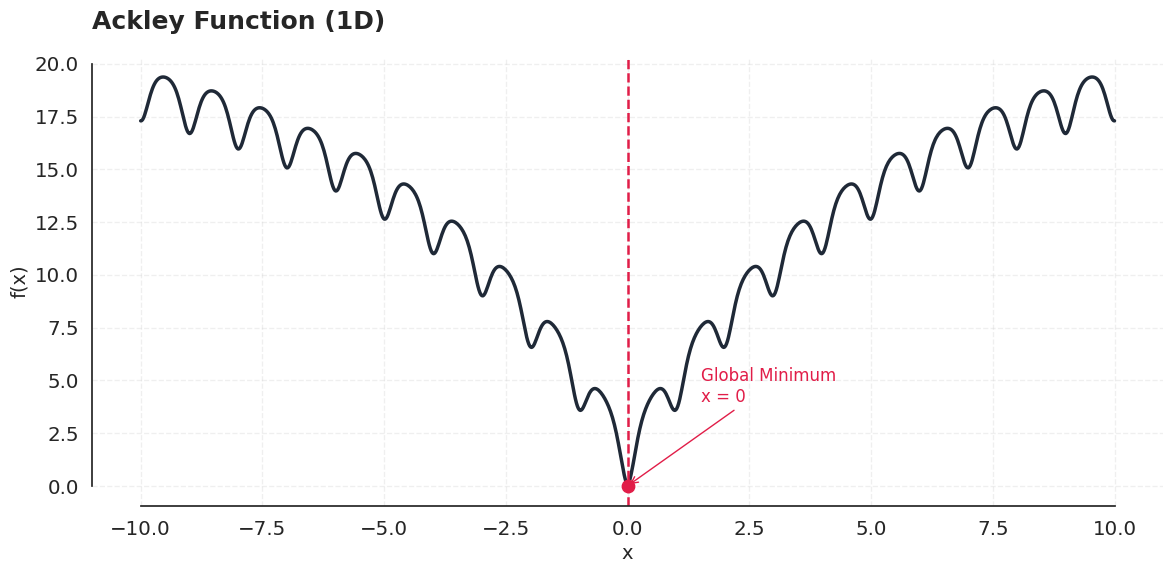
\includegraphics[width=\textwidth]{weeks_new/imgs/multi_mod.png}
    \caption{One-dimensional and multi-modal optimization problem}
    \label{fig:multi_mod}
\end{figure}

As seen in the figure above, a multi-modal function may have multiple peaks (maxima) and valleys (minima). Optimization algorithms may get stuck in a local optimum depending on the starting point and fail to find the global optimum. Therefore, metaheuristic methods may be preferred to find the global optimum, especially in complex engineering problems. 